\begin{frame}
  \frametitle{A trapezoidal acoustic wave is used to study the physics}
  \begin{figure}%
    \centering%
    \def\svgwidth{\textwidth}%
    {\footnotesize
    \import{./figs/}{shock-us_2_trapz_labels_logic.pdf_tex}%
    }
  \end{figure}
  \begin{itemize}
  \item Symmetric in time
  \item Returns to ambient pressure
  \item Well-prescribed pressure gradients
  \end{itemize}
\end{frame}
%
\begin{frame}\frametitle{\vspace*{0.5cm} Base case: a $10$ MPa trapezoidal wave hits the sinusoidal interface}%
  %
  \hfill%
  %
  \begin{minipage}{0.48\textwidth}
    \begin{figure}
      \centering
      \hfill%
      \def\svgwidth{0.75\textwidth} {\footnotesize
        \import{../figs/lung_figs/}{domain_bcs2.pdf_tex}%
      }%
      \hfill%
    \end{figure}
  \end{minipage}
  %
  \hfill%
  %
  \begin{minipage}{0.48\textwidth}
    \begin{figure}
      \centering%
      \hfill%
      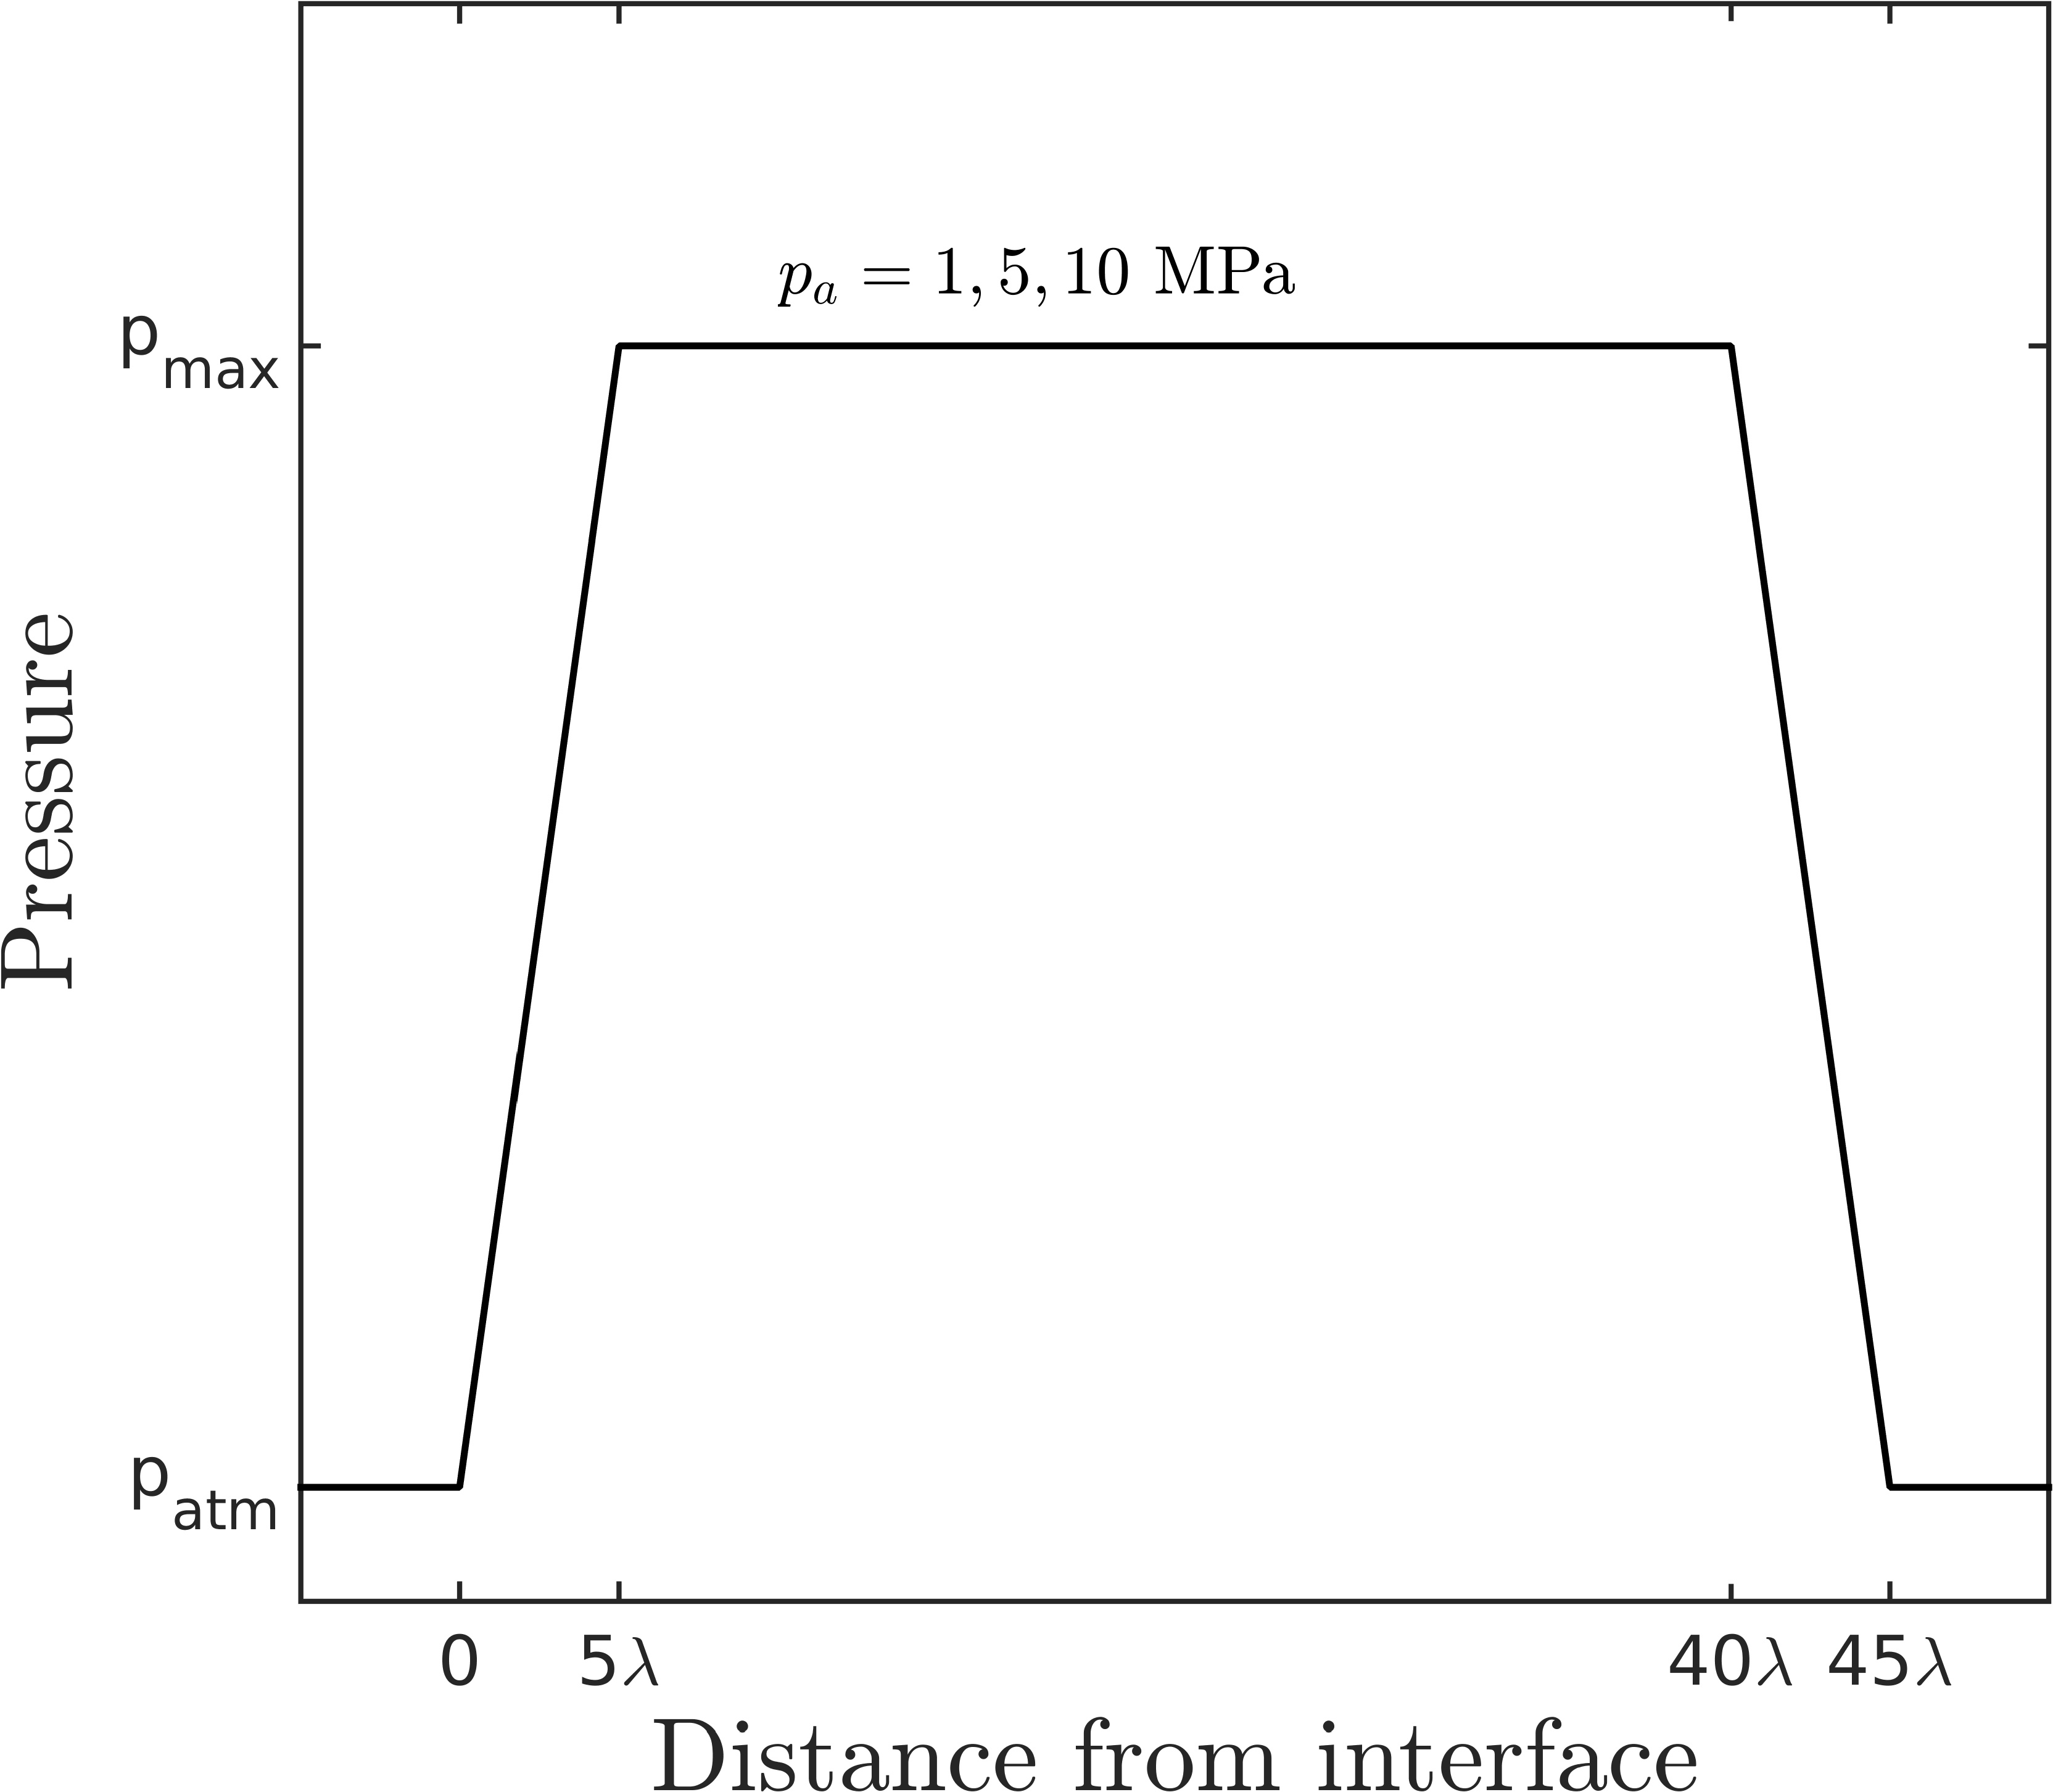
\includegraphics[width=\textwidth]{../figs/lung_figs/p0_vs_y}%
      \hfill%
    \end{figure}
  \end{minipage}
  %
  \hfill%
  %
\end{frame}




%%% Local Variables:
%%% mode: latex
%%% TeX-master: "main"
%%% End:
